\documentclass[tikz,border=5pt,12pt]{standalone}
\usepackage{tikz}

\begin{document}    
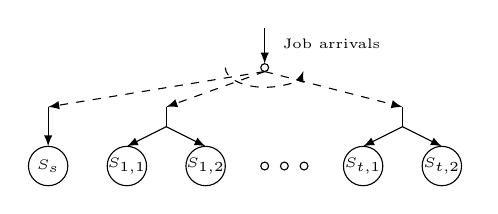
\begin{tikzpicture}[>=latex]

\draw[->] (2.75,0.75) -- (2.75,0.30);
\node at (3.6,0.55) {\tiny Job arrivals};
\draw (2.75,0.25) circle [radius=0.05] node {};
\draw [->,dashed] (2.25,0.25) arc[x radius=0.5, y radius =0.25, start angle=-180, end angle=-10];
\draw[dashed,->] (2.75,0.2) -- (0,-0.25);
\draw[dashed,->] (2.75,0.2) -- (1.5,-0.25);
\draw[dashed,->] (2.75,0.2) -- (4.5,-0.25);

\draw[->] (0,-0.25) -- (0,-0.75);
\draw (0,-1) circle [radius=0.25] node {\tiny $S_s$};

\draw[-] (1.5,-0.25) -- (1.5,-0.5);
\draw[->] (1.5,-0.5) -- (1,-0.75);
\draw[->] (1.5,-0.5) -- (2,-0.75);
\draw (1,-1) circle [radius=0.25] node {\tiny $S_{1,1}$};
\draw (2,-1) circle [radius=0.25] node {\tiny $S_{1,2}$};

\draw (2.75,-1) circle [radius=0.05];
\draw (3,-1) circle [radius=0.05];
\draw (3.25,-1) circle [radius=0.05];

\draw[-] (4.5,-0.25) -- (4.5,-0.5);
\draw[->] (4.5,-0.5) -- (4,-0.75);
\draw[->] (4.5,-0.5) -- (5,-0.75);
\draw (4,-1) circle [radius=0.25] node {\tiny $S_{t,1}$};
\draw (5,-1) circle [radius=0.25] node {\tiny $S_{t,2}$};

\end{tikzpicture}
\end{document}